% !TeX root = ../thuthesis-example.tex

\chapter{PERFORMANCE TESTING AND USABILITY EVALUATION OF THE VR-IOT RESEARCH PLATFORM}

In this chapter Smart home, one of the most common IoT environments, is used for research on creating a device of a new type. There are several devices in the example configuration (Figure~\ref{fig:TestingEquipment-figure}):
\begin{enumerate}
    \item A Smart Wi-Fi lamp;
    \item A PC running openHAB server and NUIX-Studio App instance;
    \item A PC running NUIX-Studio App instance;
    \item An Oculus Quest VR Headset;
    \item A smart vacuum cleaner.
\end{enumerate}

\begin{figure}
  \centering
  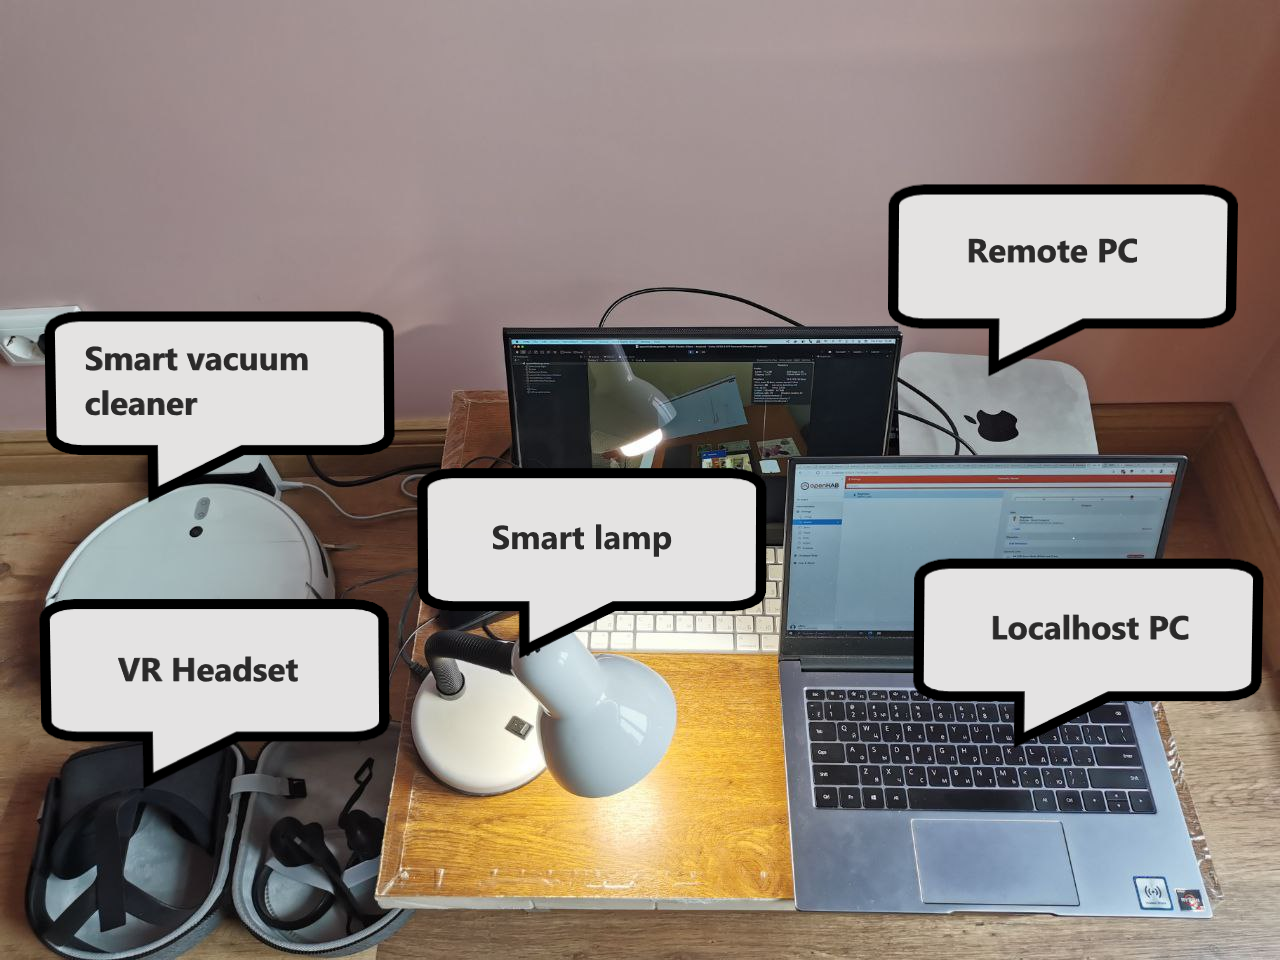
\includegraphics[width = 0.9 \linewidth]{figures/TestingEquipment.png}
  \caption{Testing equipment.}
  \label{fig:TestingEquipment-figure}
\end{figure}

The example research is on adding gesture control functionality for the smart lamp\footnote{Smart vacuum cleaner and remote PC will be used in the next experiment}.

The virtual environment provides Widgets for Light and Gesture Recognition. In other words, a virtual lamp should be equivalent to the real-world one and gesture interface should be implemented.

\section{Server setup}
Firstly, a binding needs to be added to the openHAB server. Xiaomi Mi IO binding makes it possible to automatically add the Xiaomi Smart Wi-Fi Lamp to the server (Figure~\ref{fig:ServerSetupProcedure-figure}).

\begin{figure}
  \centering
  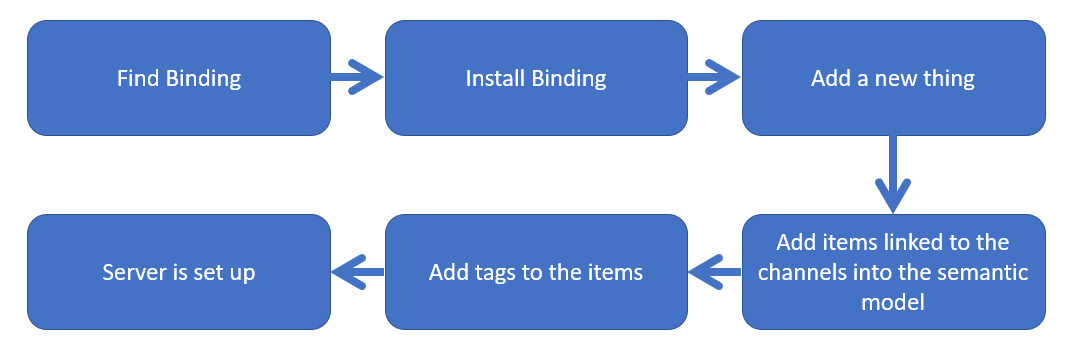
\includegraphics[width = 0.9 \linewidth]{figures/ServerSetupProcedure.png}
  \caption{Server setup procedure.}
  \label{fig:ServerSetupProcedure-figure}
\end{figure}

Next is adding items linked to the lamp channels. In the example the lamp brightness dimmer is added to the semantic model.

\begin{figure}
  \centering
  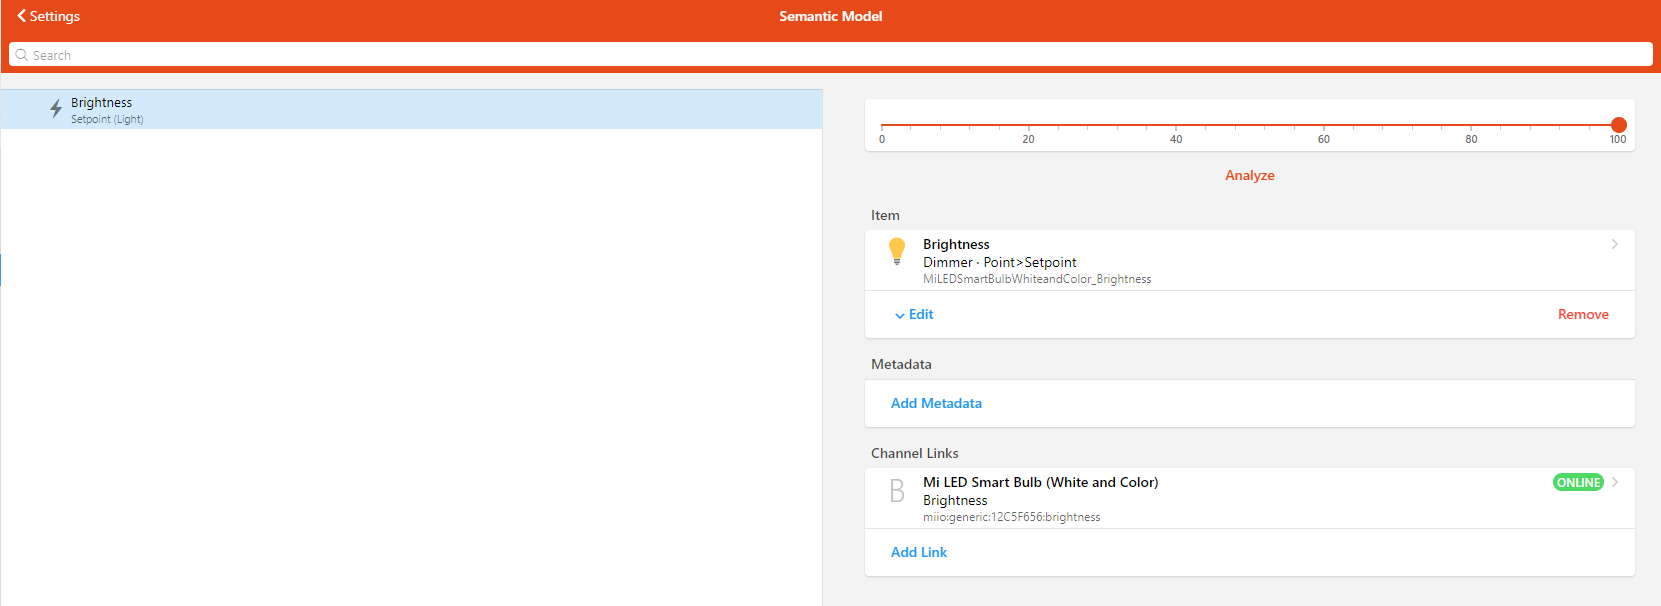
\includegraphics[width = 0.9 \linewidth]{figures/SemanticModelOne.png}
  \caption{Semantic model 1.}
  \label{fig:SemanticModelOne-figure}
\end{figure}

As seen on Figure~\ref{fig:SemanticModelOne-figure}, the brightness can be already controlled by moving the dimmer. The real-world lamp will change the brightness based on the value on the server.

Next step is adding tags to the item:the lamp should be controlled by Gestures, then a corresponding tag has to be added (Figure~\ref{fig:ItemEditPage-figure}).

\begin{figure}
  \centering
  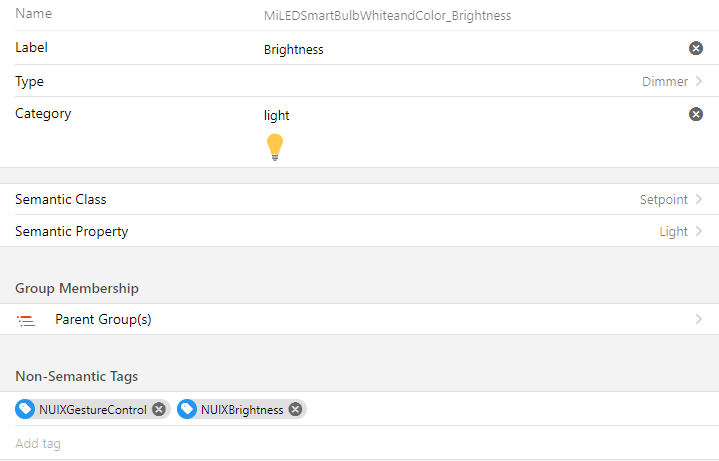
\includegraphics[width = 0.9 \linewidth]{figures/ItemEditPage.png}
  \caption{Item Edit Page.}
  \label{fig:ItemEditPage-figure}
\end{figure}

The server has been set up for connection to NUIX-Studio App instances.

\section{Running NUIX-Studio APP}

After the server has been set up, and the Smart home environment has been chosen, the platform is ready to run on the devices.

(A screenshot with gesture control).

In the experiment a VR-IoT platform user performs three tasks:
\begin{enumerate}
    \item Put on Virtual reality headset;
    \item Press the virtual button to establish a Client-Server connection and receive the items list;
    \item Perform a "Thumb up" gesture. By rotating the fist, the lamp brightness changes in the VR-IoT environment \footnote{Both in real and virtual worlds}.
\end{enumerate}

These actions were performed by the user of the platform. Thus, support for gestures was added to control the brightness of the lamp and the experiment to create a new device for the existing environment can be considered a success.

\section{Performance analysis}

The analysis of platform performance is not the main goal of the study, but nevertheless, it is indicative in terms of finding bottlenecks. It will be shown that it makes sense to perform rendering tasks on a separate server, and having a common database for all instances of the application will help to achieve in the end the simultaneous work of several users within the system.

The first experiment is the analysis of the system startup, performed on three devices by registering the startup time (Figure~\ref{fig:SystemStartupScheme-figure}).

\begin{figure}
  \centering
  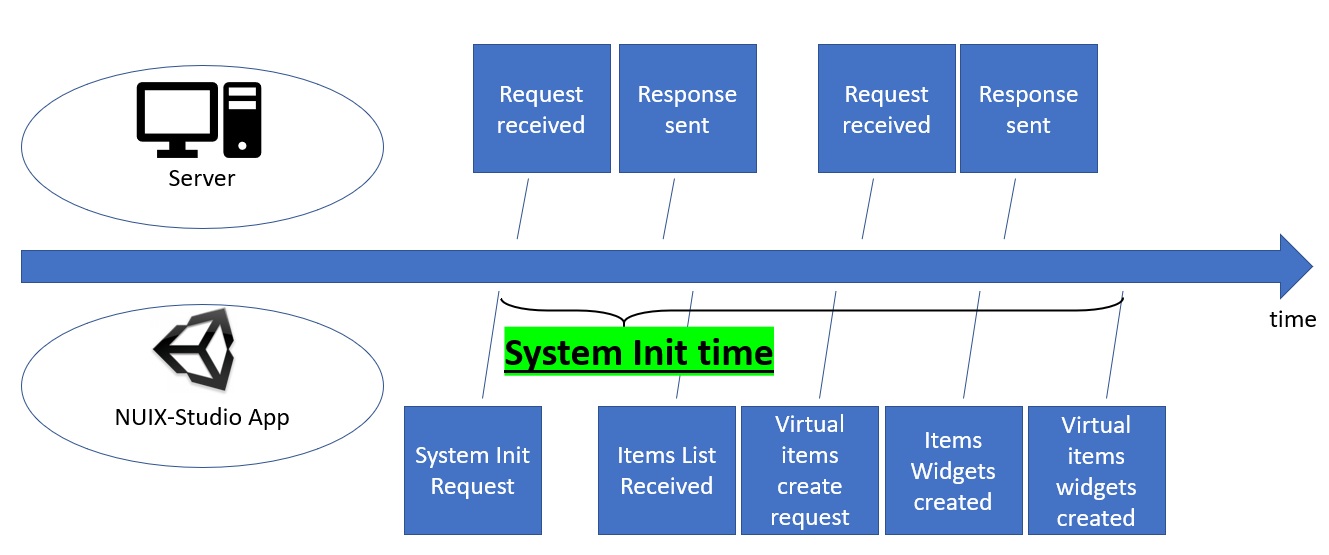
\includegraphics[width = 0.9 \linewidth]{figures/SystemStartupScheme.png}
  \caption{System startup scheme.}
  \label{fig:SystemStartupScheme-figure}
\end{figure}

The hardware specifications can be seen on Table~\ref{tab:hardware-specifications-table} \footnote{Localhost PC is a notebook running openHAB server as well as one instance of NUIX-Studio APP; Remote PC is a computer running one instance of NUIX-Studio APP and connected to the same Wi-Fi network as localhost PC; Oculus Quest is a Virtual Reality Headset running NUIX-Studio APP and connected to the same Wi-Fi network as PCs.}.

\begin{table}
  \centering
  \begin{threeparttable}[c]
    \caption{Hardware specifications in the experimental setup}
    \label{tab:hardware-specifications-table}
    \begin{tabular}{ll}
      \toprule
      Unit    &         Specifications                 \\
      \midrule
      Localhost PC & Ryzen 5 3500u, Windows 10 \\
      Remote PC & Core i5 4278U, macOS 11.2.3    \\
      Oculus Quest        & Qualcomm Snapdragon 835, Android-based            \\
      \bottomrule
    \end{tabular}
  \end{threeparttable}
\end{table}

Each test was performed on a new instance of Unity APP to avoid cashing influence. And then mean values have been calculated (Figure~\ref{fig:SystemInitTime-figure}).

\begin{figure}
  \centering
  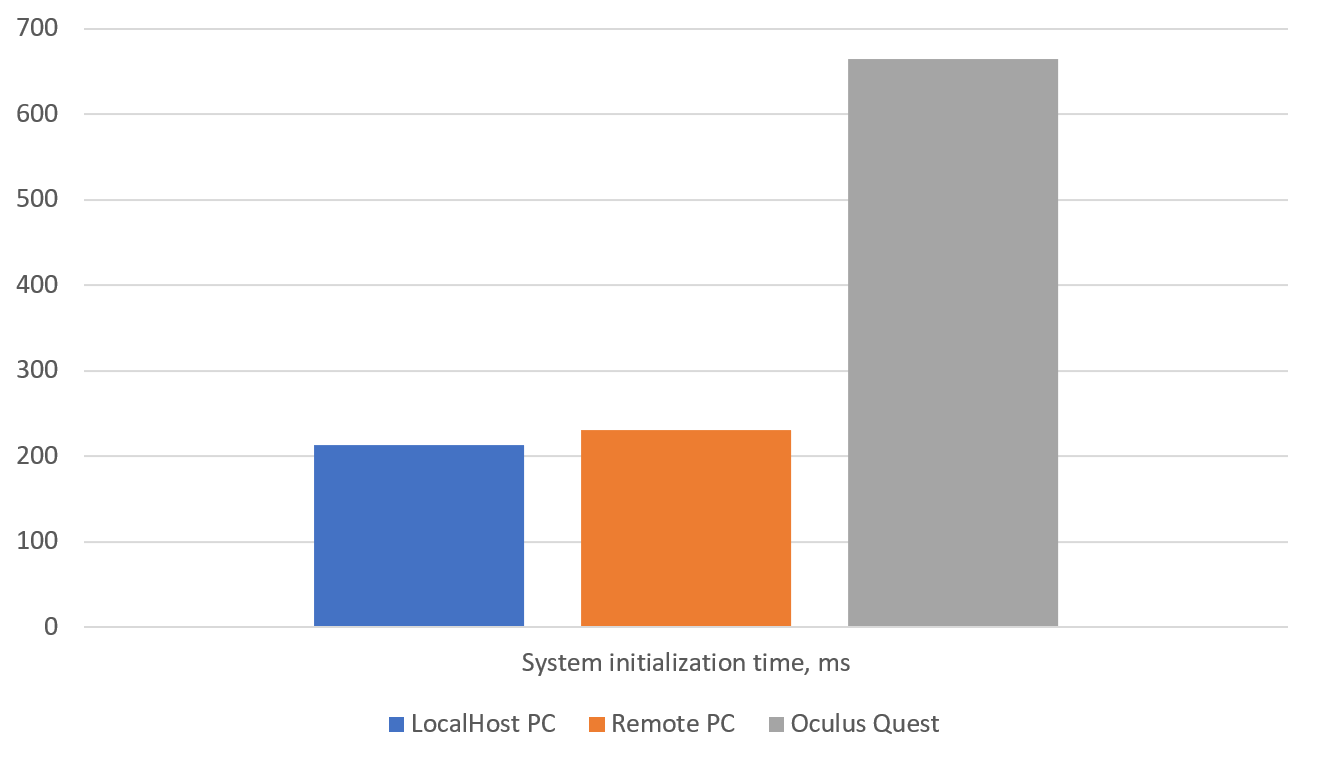
\includegraphics[width=0.9\linewidth]{figures/SystemInitTime.png}
  \caption{System initialization time measured on different client devices.}
  \label{fig:SystemInitTime-figure}
\end{figure}

As seen on Figure~\ref{fig:SystemInitTime-figure}, the system initialization time is a time-consuming operation, which from 200 to over 600ms in average to perform.

In the next experiment, event processing time was measured. On one of the devices running the NUIX-Studio App instance, the Item \footnote value changed{In this case, the brightness of the smart bulb changed by moving the corresponding pinch slider widget}. The server processed the received request to change the Item parameter, and an Event containing information about the new Item value was sent to all devices connected to the server, running NUIX-Studio App Instance. The device on which this Item change occurred ignored the new incoming value because it is the same as the old value. The measurement object is the processing time of a request on another device (Figure~\ref{fig:EventProcessingScheme-figure}).

\begin{figure}
  \centering
  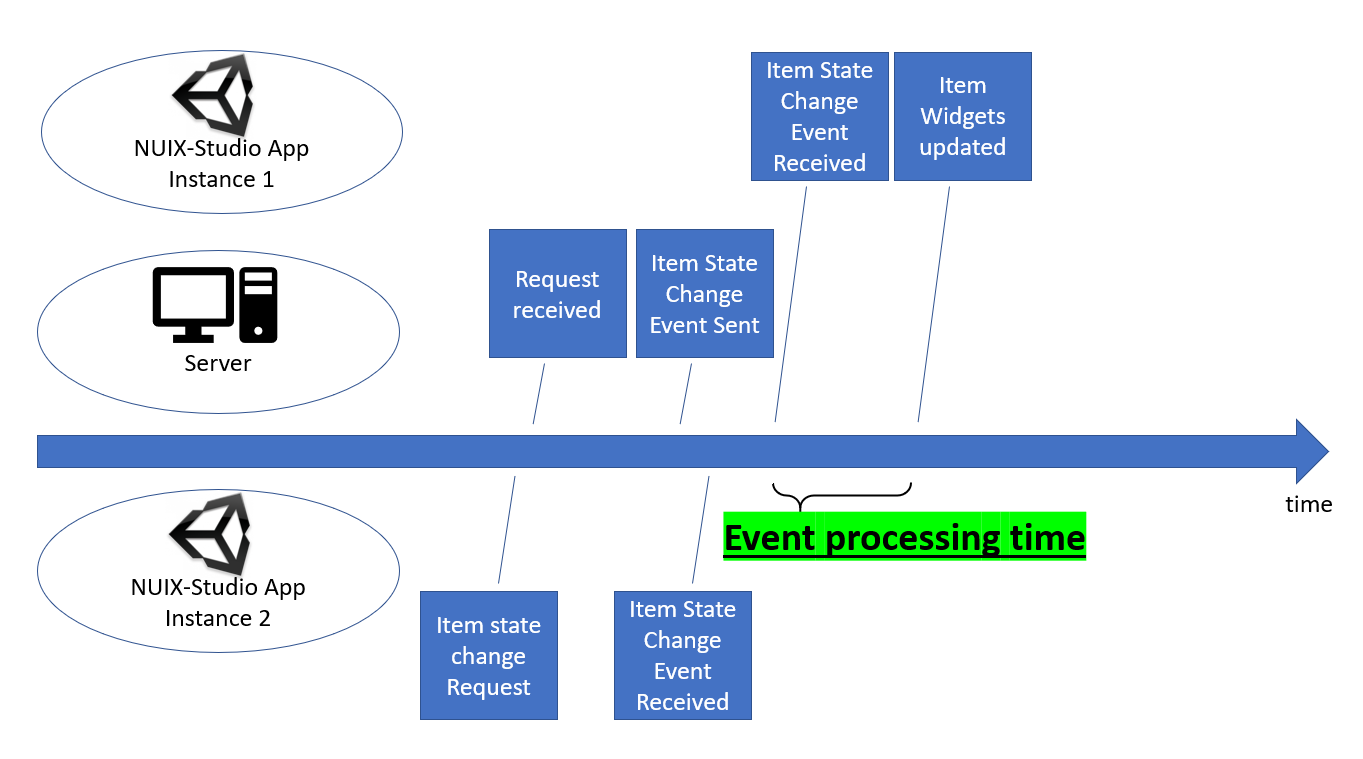
\includegraphics[width = 0.9 \linewidth]{figures/EventProcessingScheme.png}
  \caption{Event processing scheme.}
  \label{fig:EventProcessingScheme-figure}
\end{figure}

\begin{figure}
  \centering
  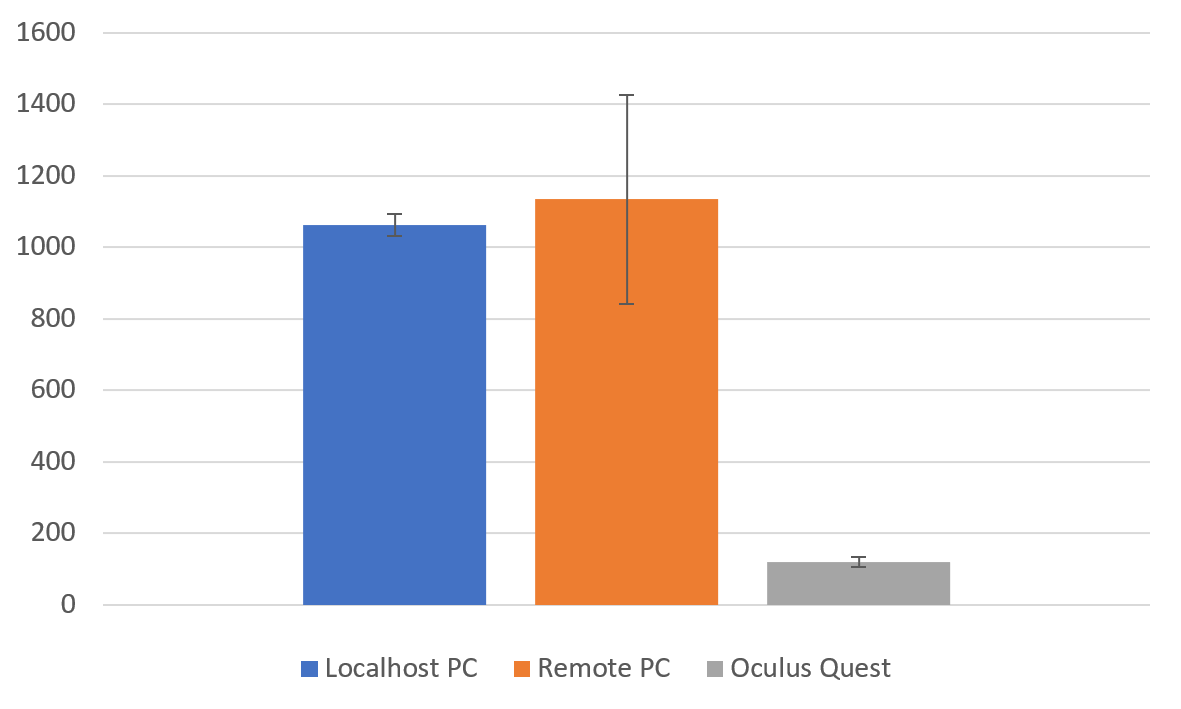
\includegraphics[width = 0.9 \linewidth]{figures/EventProcessingTime.png}
  \caption{Event processing time measured on different devices.}
  \label{fig:EventProcessingTime-figure}
\end{figure}

As you can see from the resulting histogram (Figure~\ref{fig:EventProcessingTime-figure}), Oculus Quest performance on this test is outstanding:the event processing time is around 10 times lower compared to the PCs, which stands in confrontation with the assumption that this test is only device performance-based. One of the possible reasons of such results is optimization:NUIX-Studio APP is built for Oculus Quest, while on PCs it is run in the “Editor” mode, not built specifically for the platform.


The results of this experiment will be used in the future: system initialization time is time consuming and is based on the device hardware performance, and in some later experiments it is better to not perform time calculations that include system initialization, while event processing time is relatively low, and in most cases it can be neglected.

The next experiment uses a virtual reality headset, a smart light bulb, and a server running an application on it. Suppose that a light sensor is used inside the smart home system, which is located at a relatively large distance from the lamp (2-3 meters), and is triggered when the amount of light falling on its sensor exceeds a certain threshold. For example, this setup is sometimes used in factories when initially setting up lighting to find the line between a comfortable level of lighting and an optimal level of energy consumption. The light sensor will be triggered precisely at some sufficiently large value of the lamp brightness. Thus, you need the most accurate adjustment of the brightness level of the light bulb.

In a previous experiment, it was shown that gesture control is possible to control the brightness level of a lamp. Let us show that in this case, the transfer of computations from the helmet of virtual reality to the server is necessary. The user assignment consists of the same steps as in the previous experiment, but it adds one more step:fine tuning the brightness level. Suppose that the light sensor is triggered at a light bulb brightness level of 50 out of 100 \footnote{This number was chosen by the author of the study at random, without relying on the principles of fits law}. The user's task is to bring the brightness of the light bulb to this position as quickly as possible using gesture control. In order to exclude additional operations not related to the direct use of gestures to change the brightness of the lamp, such as starting the system, the subject had to repeat the step with bringing the brightness of the lamp to the specified position two times. The time between the first and second times, when the lamp brightness was equal to the specified value, can be divided into two components (Equation \eqref{eq:totaltime}):the reaction time of the test subject to a successful change in the brightness level $ t_{foc} $, and the execution time of the new calibrations $ t_{cal} $.

\begin{equation}
  t = t_{foc} + t_{cal}
  \label{eq:totaltime}
\end{equation}

The experiment involved five people. Two series of experiments were carried out:in the first series, the lamp illumination was counted on a virtual reality device, and in the second, on a server. Only information, namely a map of light, was transmitted to the virtual reality device. In each series of experiments, twenty-five measurements were made, and the data obtained were plotted on the graph (). If we take into account that the focusing time of the experimental $ t_{foc} $ is a value independent of the changed synchronization parameters, then the difference between the calculated time in the first and second series of experiments will just be equal to the difference between the time spent on calibrating the lamp brightness in the first and the second series of experiments. (Equation \eqref{eq:totaltime})

\begin{equation}
  t _{\delta} = (t_{foc} + t_{cal_1}) - (t_{foc} + t_{cal_1}) = t_{cal_1} - t_{cal_2}
  \label{eq:deltatime}
\end{equation}

As you can see from the resulting histogram, the difference when performing the calibration function in the first and second tasks is 500 milliseconds. Considering that the processing time of a request coming from the server is no more than 1 millisecond \footnote{It was obtained in the previous chapter}, there is a huge difference in execution time.

During the experiment, additional data was also analyzed, such as the number of frames per second with which the image was drawn on the screen. The graph () shows that in the first series of experiments the number of frames per second drops significantly as soon as the system is initialized and widgets for items from semantic model are created:from 72 frames per second, which is a hardware limitation of the virtual reality helmet to 20 frames per second ... In the second series of experiments, such a drop is no longer observed (link to the graph):due to the fact that the lighting is counted on a separate device, the number of frames per second drops only slightly from 72 to 65. Considering that hands recognition is processed no more than once per second. frame, then we can make the assumption that the time difference is just due to the delay in reading the gesture. You can draw an analogy with a mouse:the user will get to the desired button more often if the mouse control is more responsive. However, the main challenge of the experiment was to show how transferring resource-intensive computing from a VR headset to a server improves user experience, one of the requirements for building a VR-IoT Research platform. Thus, the experiment can be considered successful.


In the next experiment, the hypothesis was tested whether it is possible to work together in one VR-IoT environment by adding new IoT devices to the system and changing their parameters. The author does not dwell in detail on the discussion of this hypothesis, since its results have already been predicted from previous experiments:
\begin{enumerate}
    \item The time for adding a device to the system is limited by the performance of a specific platform, as well as by the speed of the Internet connection within the Wi-Fi network. When running 300 sequential ping tests from remote PC to localhost PC, all the values ​​obtained were less than 100ms, with 90 percent values ​​ranging from 45ms to 70ms. The time spent by the device on creating widgets for a smart vacuum cleaner roughly corresponded to the time of system initialization;
    \item The time from changing Item to remote PC NUIX-Studio App Intance until remote PC received confirmation of the corresponding widgets on localhost PC NUIX-Studio App Instance did not exceed 60ms, with 90 percent of values ​​from 53ms to 80ms.
\end{enumerate}

Thus, the speed of the network plays a significant role in the operation of the system. Only with the minimal network latency available now in Wi-Fi 6 networks, as well as in 6G networks in the future, will simultaneous work inside the same VR-IoT environment be hampered. However, it has been observed that operations such as adding new devices to the system are time consuming. Due to the fact that there is a request to create game objects, the author assumes that the main delay is associated precisely with the internal processes inside the Unity 3D engine.

The next chapter will show you how you can theoretically work around these limitations.